\section{Diversity im Reinforcement Learning}
\label{sec:diversity}
% Ziel
In diesem Kapitel beschäftigen wir uns damit, wie das Konzept von Diversity im Bereich des Reinforcement Learning (RL) Anwendung finden kann. Ziel ist, dass ein RL Agent in einer unüberwachten Phase zunächst Fähigkeiten erlernt, welche das Bewältigen von Aufgaben in der darauf folgenden, überwachten Phase erleichtern sollen.

Dieses Kapitel stützt sich zu einem Großteil auf die wissenschaftliche Arbeit \textit{Diversity is all you need: Learning skills without a reward function}\cite{diversity_eysenbach}. Falls nicht anders angegeben, wurden die Informationen hieraus entnommen.

% Grundlegende Begriffe
\subsection{Klärung wichtiger Begriffe aus der Informationstheorie}
\label{sec:informationtheory}
Im Folgenden werden Begriffe aus der Informationstheorie verwendet, welche es zunächst zu klären gilt. Wir betrachten \textit{Entropie} und \textit{Transinformation} nach \cite{elements_cover} und \cite{information_werner}.

\smallspace

Die \textit{Entropie} beschreibt in der Informationstheorie den mittleren Informationsgehalt bzw. die Ungewissheit einer Quelle. Ist beispielsweise bei einer Ereignismenge jedes Ereignis gleich wahrscheinlich, so ist die Ungewissheit maximal \cite{information_werner}.

Nach \cite{elements_cover} besitzt eine diskrete Zufallsvariable $ X $ mit dem Zeichenvorrat $ \mathcal{X} $ und der Wahrscheinlichkeitsfunktion $ p(x) $ die \textit{Entropie}
\begin{equation*}
    H(X) = -\sum_{x \in \mathcal{X}} p(x) \cdot log\ p(x) \label{eq:entropy}
\end{equation*}

Diese lässt sich nach \cite{elements_cover} auch über den Erwartungswert $ E $ berechnen unter Verwendung von
\begin{equation*}
    H(X) = E_p\ log\ \frac{1}{p(X)} \label{eq:entropy_1}
\end{equation*}
, woraus unter Anwendung der Rechenregeln für Logarithmus und Erwartungswert trivial
\begin{equation}
    H(X) = - E_p\ log\ p(X) \label{eq:entropy_2}
\end{equation}
folgt.

Desweiteren ist die Formel für die \textit{bedingte Entropie} nach \cite{elements_cover} gegeben durch
\begin{equation}
    H(Y|X) = - E_{p(x,y)}\ log\ p(Y|X) \label{eq:condit_entropy}
\end{equation}

\smallspace

Die \textit{Transinformation} beschreibt die Menge an Information, die eine Zufallsvariable über eine andere enthält bzw. die Reduktion der Ungewissheit aufgrund des Wissens um die jeweils andere Zufallsvariable \cite{elements_cover}.

Mathematisch wichtig für uns ist lediglich der Zusammenhang zwischen \textit{Transinformation} und \textit{Entropie}, welcher nach \cite{elements_cover} gegeben ist durch
\begin{equation}
    I(X;Y) = H(X) - H(X|Y) = H(Y) - H(Y|X) \label{eq:trans_ent}
\end{equation}

% Erklärung des Algorithmus
\subsection{Funktionsweise}
\label{sec:howitworks}
\begin{figure}
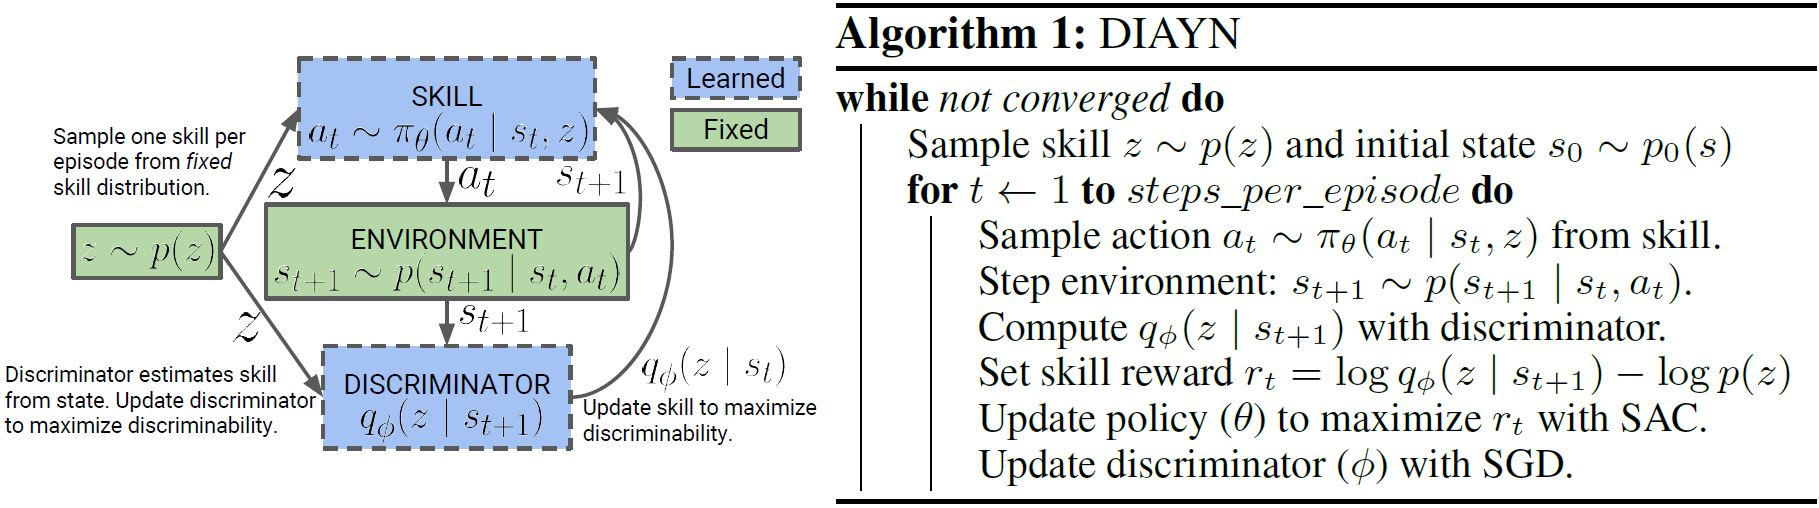
\includegraphics[width=\textwidth, keepaspectratio=true]{images/algorithm_diayn.JPG}
\caption{``Diversity is all you need'' Algorithmus} \label{img:diayn}
\source{\cite{diversity_eysenbach}}
\end{figure}
Das selbstständige Erlernen von brauchbaren Fähigkeiten, so wie in \cite{diversity_eysenbach} beschrieben, baut auf drei Grundideen auf.

\smallspace

(1) Unterschiedliche Fähigkeiten sollten andere Zustände besuchen, sodass ihre Unterscheidbarkeit gewährleistet ist.

%TODO "Paper"
(2) Um besagte Fähigkeiten zu unterscheiden, werden nicht die Aktionen, sondern die Zustände betrachtet. Das liegt daran, dass Aktionen, welche die Umgebung nicht beeinflussen, für einen Beobachter nicht erkennbar sind. Das Paper verdeutlicht dies mit einem treffenden Beispiel. Für einen außenstehenden Betrachter ist nicht ersichtlich, wie fest ein Roboterarm eine Tasse in der Hand hält, falls sich diese nicht bewegt.

(3) Schließlich soll erreicht werden, dass die Fähigkeiten so vielfältig (\textit{diverse}) wie möglich sind. Die Idee ist, dass unterscheidbare Fähigkeiten mit einer hohen Entropie einen Zustandsraum abdecken, welcher sich weit entfernt von anderen Fähigkeiten befindet.

\smallspace

Um diese Punkte zu realisieren, definieren wir zunächst die Zufallsvariablen $ S $ und $ A $ für Zustände und Aktionen. Sei nun $ Z \sim p(z) $ eine latente Variable, unter deren Bedingung die Strategie definiert wird. Bei fixem $ Z $ sprechen wir hier von einer "Fähigkeit". Entropie sowie Transinformation werden zur Basis $ e $ berechnet.

Nun soll die Transinformation zwischen Fähigkeiten und Zuständen, $ I(S;Z) $, maximiert werden um sicherzustellen, dass die Fähigkeit die vom Agent durchlaufenen Zustände vorgibt. Anders gesagt wird sichergestellt, dass aus den besuchten Zuständen auf die Fähigkeit geschlossen werden kann.

Außerdem minimieren wir die Transinformation zwischen Fähigkeit und Aktionen bei gegebenen Zustand, $ I(A; Z | S) $. So wird garantiert, dass nicht Aktionen, sondern Zustände für die Unterscheidung von Fähigkeiten verwendet werden.

% unklar
Maximiert wird auch die Entropie $ H(A|S) $.

\smallspace

Insgesamt maximieren wir nach \cite{diversity_eysenbach} also
\begin{align}
    \mathcal{F}(\theta) &\stackrel{\triangle}{=} I(S;Z) + H(A|S) - I(A;Z|S) \label{eq:objective_1}\\
    & = (H(Z) - H(Z|S)) + H(A|S) - (H(A|S) - H(A|S,Z)) \nonumber\\
    & = H(Z) - H(Z|S) + H(A|S,Z) \label{eq:objective_intuitive}
\end{align}
Der Term wurde unter Verwendung von \eqref{eq:trans_ent} umgeformt.

Da sich $ p(z|S) $ nicht genau berechnen lässt, wird das Folgende mit einem discriminator $ q_\phi $ approximiert. Mit der Jensenschen Ungleichung haben wir laut \cite{diversity_eysenbach} eine untere Schranke $ \mathcal{G}(\theta) $ für $ \mathcal{F}(\theta, \phi) $:
\begin{align}
    \mathcal{F}(\theta) & = H(A|S,Z) - H(Z|S) + H(Z) \nonumber\\
    & = H(A|S,Z) + E_{z \sim p(z), s \sim \pi(z)}(log\ p(z | s)) - E_{z \sim p(z)}(log\ p(z)) \label{eq:objective_2}\\
    & \ge H(A|S,Z) + E_{z \sim p(z), s \sim \pi(z)}(log\ q_\phi(z | s) - log\ p(z)) \stackrel{\triangle}{=} \mathcal{G}(\theta, \phi) \nonumber
\end{align}
In \eqref{eq:objective_2} wurden die Entropien nach \eqref{eq:entropy_2} und \eqref{eq:condit_entropy} umgeformt.

\smallspace

Nach der unüberwachten Trainingsphase verfügt der Agent über eine Sammlung von verschiedenartigsten Fähigkeiten, von denen vermutlich einige nutzlos sind. Aufgrund der implementierten Diversity müssen jedoch Fähigkeiten existieren, welche sich stark von den unbrauchbaren unterscheiden. So ist es intuitiv einleuchtend, dass es sich hierbei um sinnvolle Fähigkeiten handelt.

%\newpage
% Beispiele
\subsection{Experimente und Beispiele}
\label{sec:examplesdiversity}
\begin{figure}[h]
\begin{subfigure}{0.41\textwidth}
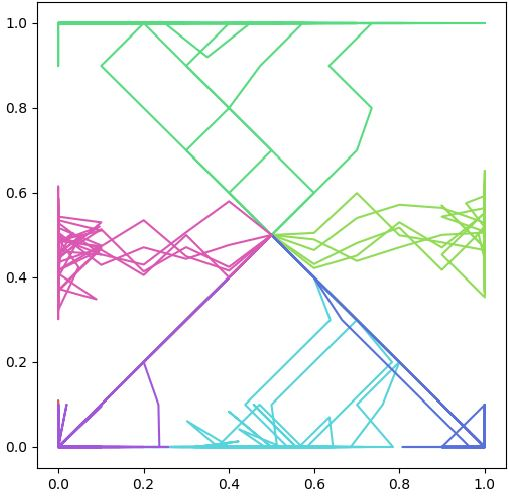
\includegraphics[width=0.95\textwidth]{images/example_diayn_1.JPG}
\caption{Zweidimensionale Navigation} \label{img:diayn_ex1}
\end{subfigure}
\begin{subfigure}{0.59\textwidth}
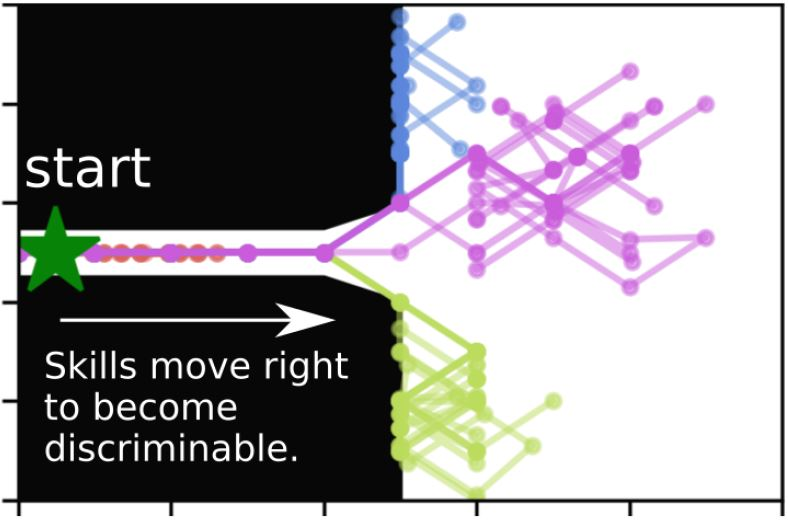
\includegraphics[width=0.95\textwidth, right]{images/example_diayn_2.JPG}
\caption{Überlagernde Fähigkeiten} \label{img:diayn_ex2}
\end{subfigure}
\caption{TODO} \label{img:diayn_ex}
\source{\cite{diversity_eysenbach}}
\end{figure}

Wie bereits mehrfach angemerkt ist das Ziel das eigenständige Erlernen von vielfältigen Fähigkeiten. \cite{diversity_eysenbach} liefert zunächst das simple Beispiel einer zweidimensionalen Navigation in einem leeren Raum \ref{img:diayn_ex1}. Hier ist sehr anschaulich zu erkennen, wie die farblich kodierten Fähigkeiten unterschiedliche Zustandsräume abdecken.

Einen Schritt weiter gedacht zeigt das Beispiel \ref{img:diayn_ex2}, dass sich Fähigkeiten unter Umständen auch zeitweilig überlagern können, solange sie schlussendlich unterscheidbare Zustandsräume abdecken.

\smallspace

% WICHTIG
In beiden Beispielen ist gut zu erkennen, wie sich die Fähigkeiten gegenseitig ``abstoßen'' und so automatisch ein Großteil des Zustandsraums abgedeckt wird. Die erkundeten Zustände liegen außerdem gleichmäßig über dem Zustandsraum verteilt.

\smallspace

\begin{figure}[h]
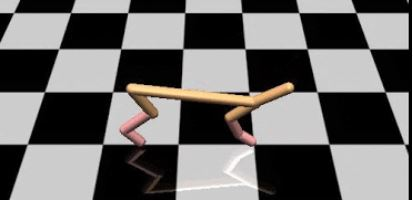
\includegraphics[width=0.5\textwidth, keepaspectratio=true, center]{images/cheetah_image.JPG}
\caption{Experiment ``Half Cheetah''} \label{img:cheetah_ex}
\source{\cite{diversity_web}}
\end{figure}

Interessanter wird es bei den komplexeren Versuchsaufbauten. Wir betrachten im Folgenden den vom Paper \cite{diversity_eysenbach} als ``Half Cheetah'' betitelten Agenten. Hierbei handelt es sich um ein hundartiges, zweidimensionales Wesen, welches die Kontrolle über sein Vorder- und Hinterbein besitzt (siehe \ref{img:cheetah_ex}).

Ohne jegliche externe Belohnung hat dieser Agent gelernt, nach vorne und hinten zu rennen beziehungsweise zu gehen. Außerdem besitzt er die Fähigkeit, einen Vorwärtssalto zu machen. Wir empfehlen zu besseren Veranschaulichung die Einsicht der Videos auf \cite{diversity_web}.

Eine Reward-Funktion, welche ein solches Verhalten hervorruft, manuell zu definieren ist nicht einfach.

\subsection{Verwendung der gelernten Fähigkeiten}
\label{sec:diversityusage}
Nachdem nun eine Sammlung von Fähigkeiten erlernt wurde stellt sich nun die Frage, wie sich diese effektiv nutzen lässt.

\smallspace

\begin{figure}[h]
\begin{subfigure}{0.6\textwidth}
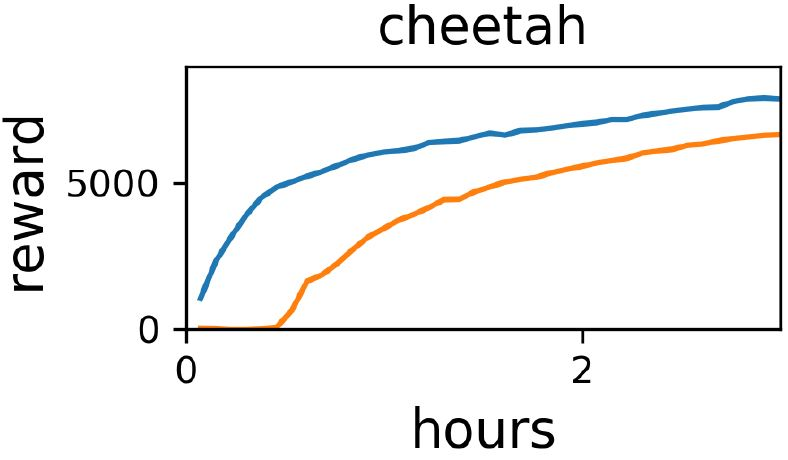
\includegraphics[width=0.8\textwidth, keepaspectratio=true, right]{images/cheetah_rewards.JPG}
\end{subfigure}
\begin{subfigure}{0.4\textwidth}
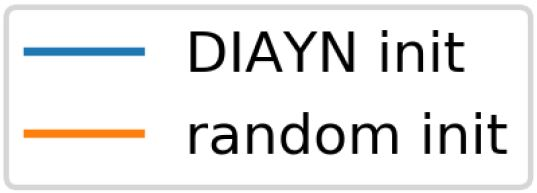
\includegraphics[width=0.5\textwidth, keepaspectratio=true, left]{images/cheetah_rewards_exp.JPG}
\end{subfigure}
\caption{Policy Initialisierung} \label{img:cheetah_rewards}
\source{\cite{diversity_eysenbach}}
\end{figure}

\cite{diversity_eysenbach} führt hier als erstes an, dass der DIAYN Algorithmus als ein Vortraining genutzt werden kann. Danach extrahiert man die Fähigkeit mit dem größten Reward und passt entsprechend die Initialgewichte der eigentlichen Policy an. \ref{img:cheetah_rewards} zeigt für das Beispiel des Half Cheetahs, dass sich bei Initialisierung mit einre vorgelernten Fähigkeit (blaue Linie) schneller größere Rewards erzielen lassen als bei einer zufälligen Initialisierung (orangene Linie).

\smallspace

Für uns interessanter ist allerdings die Verwendung für Hierarchisches Reinforcement Learning (HRL). 

Nach \cite{BerliacHierachialRL2019} lernen HRL Methoden eine Policy, welche aus mehreren Schichten besteht. Jede Ebene kontrolliert hierbei ein andere temporäre Abstraktionsebene. Dies ermöglicht es dem Agenten, nicht nur Basisoperationen auszuführen, sondern auch komplexere Aktionen wie zum Beispiel Sequenzen von Operationen einer niedrigeren Ebene.

\smallspace

\begin{figure}[h]
\begin{subfigure}{0.38\textwidth}
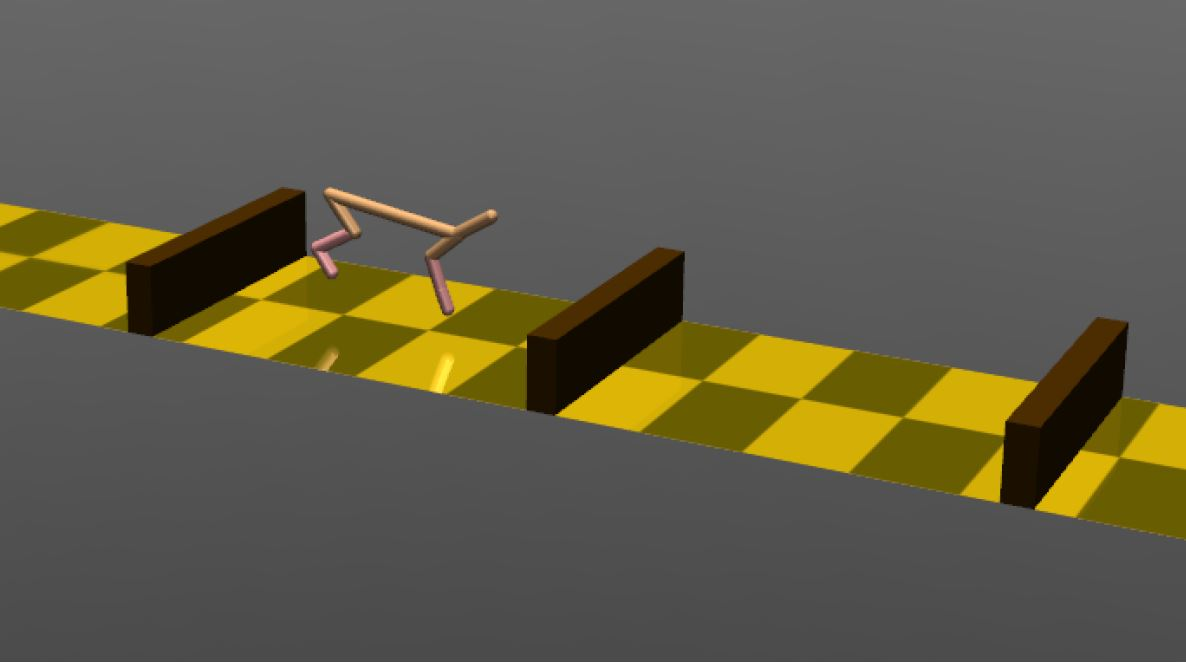
\includegraphics[width=\textwidth, keepaspectratio=true]{images/cheetah_hurdle_image.JPG}
\caption{} \label{img:cheetah_hurdle_img}
\end{subfigure}
\begin{subfigure}{0.4\textwidth}
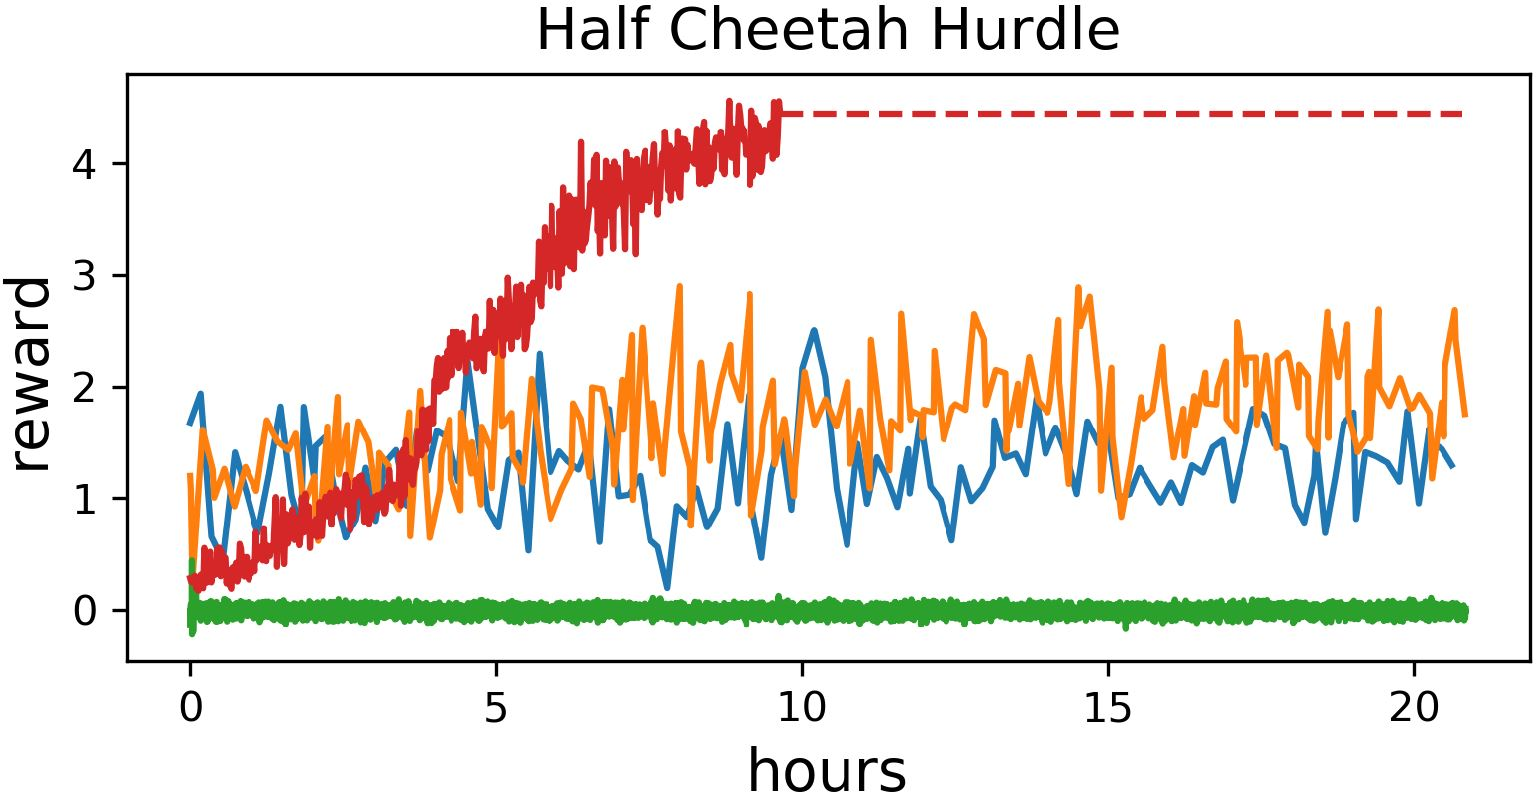
\includegraphics[width=\textwidth, keepaspectratio=true]{images/cheetah_hurdle.JPG}
\caption{} \label{img:cheetah_hurdle_graph}
\end{subfigure}
\begin{subfigure}{0.2\textwidth}
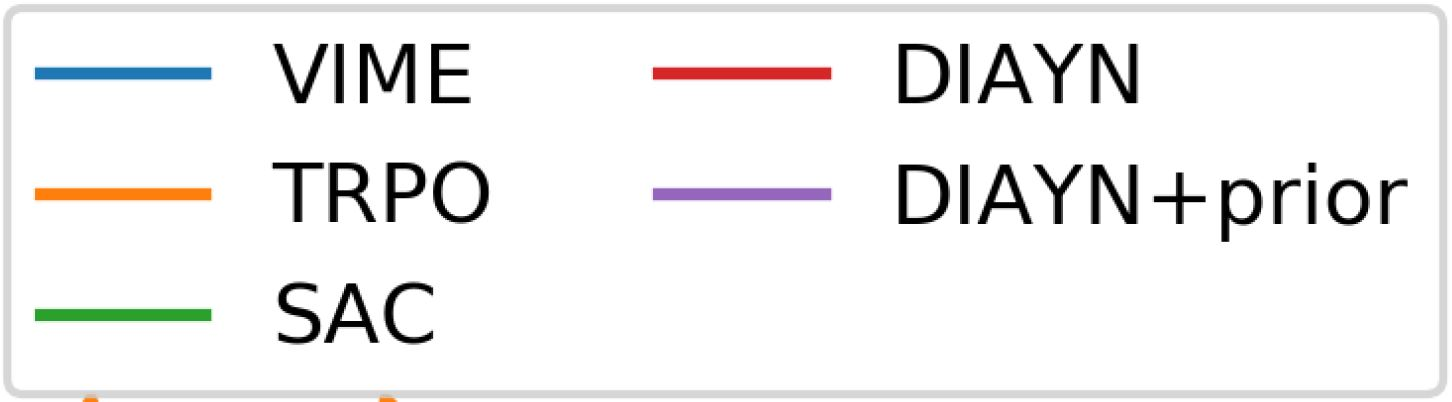
\includegraphics[width=\textwidth, keepaspectratio=true]{images/cheetah_hurdle_exp.JPG}
\end{subfigure}
\caption{DIAYN für HRL} \label{img:cheetah_hurdle}
\source{\cite{diversity_eysenbach}}
\end{figure}

Laut \cite{diversity_eysenbach} eignet sich DIAYN hervorrangend als Grundstein für HRL. Für ein Experiment diesbezüglich betrachten wir wieder den Half Cheetah. Dieser hat nun die Aufgabe, über Hürden zu springen (siehe \ref{img:cheetah_hurdle_img}) und erhält Rewards für deren überwinden.

Um die gelernten Fähigkeiten für HRL zu benutzen, wird DIAYN um einen ``meta-controller'' erweitert welcher kontrolliert, welche 10 Fähigkeiten jeweils als nächstes ausgeführt werden.

Das Experiment wird außerdem mit aktuellen Reinforcement Learning Algorithmen (VIME, TRPO und SAC) durchgeführt.

Wie die Grafik \ref{img:cheetah_hurdle_graph} zeigt, schneiden diese im Experiment sehr schlecht ab und es gibt quasi keine merkliche Steigerung des Rewards. Im Gegensatz dazu zeigt der Ansatz mit dem DIAYN Algorithmus schnell deutliche Forschritte und übertrifft merklich die anderen.

Aufgrund der Knappheit von externen Rewards gestaltet sich diese Aufgabe extrem schwierig für traditionelle RL Algorithmen. Diese müssen quasi zufällig eine Hürde übersteigen, um eine Belohnung von außen zu bekommen.

Dies zeigt nach \cite{diversity_eysenbach}, dass das eigenständige Lernen von Fähigkeiten einen effektiven Mechanismus bereit stellt, um bei Herausforderungen beim Erkunden und mit geringem externen Reward Lernerfolge zu erzielen.